
\begin{flushleft}
46
\end{flushleft}
\begin{center}
КВАНТ 1994 / № 3
\end{center}



\small
\begin{minipage}{0.3\textwidth}

алгоритм. Эта схема обладает очень полезным свойством - на каждом ее ярусе может располагаться не одна, а, вообще говоря, несколько формул (в нашем случае на первом ярусе расположены формулы $\ominus$ и $\ominus$). Расчет по этим формулам может выполняться параллельно и независимо, что может быть эффективно реализовано на различных многопроцессорных вычислительных устройствах.


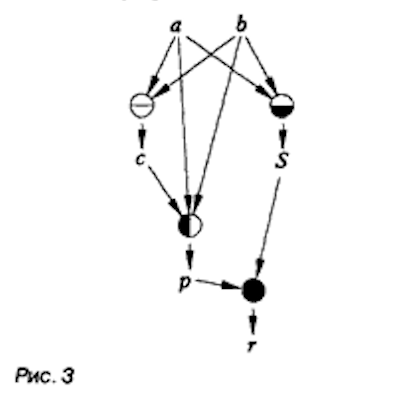
\includegraphics[scale=0.8]{images/Screenshot 2022-12-05 at 13.15.30.png}

\hspace{0.1cm} Запоминание различных формул, построение связывающей их сети, анализ
сетевой структуры, синтез решающего
алгоритма — все это по силам современ-
ным компьютерам.

\vspace{0.5cm}
\hline
\vspace{0.09cm}
\large{
Ассистирует логика 
}
\hline
\vspace{0.2cm}

\small
\hspace{0.1cm} В условиях некоторых задач наряду с
указанием, что какие-то величины принимают некие значения, говорится также о
том, что между какими-то объектами
существуют определенные отношения:
равенства, параллельности, перпендикулярности, подобия и т. д. Решение таких
задач наряду с анализом информационных связей предполагает получение каких-то логических следствий из исходных 
посылок с учетом относящихся к предмету 
аксиом и установленных теорем. На
примере следующей задачи рассмотрим,
как может быть реализован один из простейших вариантов логического вывода.


\hspace{0.1cm} Задача. Прямые s, t касаются окружности с центром в точке O соответственно
в точках A и B (рис 4). Прямые u и r
суть продолжения радиусов OA и OB.

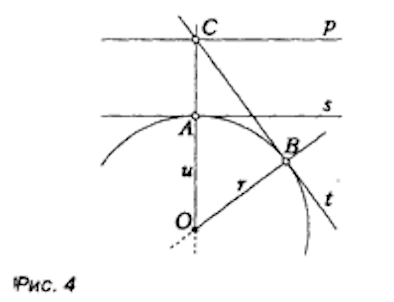
\includegraphics[scale=0.8]{images/Screenshot 2022-12-05 at 19.54.19.png}


\end{minipage}
\hspace{0.3cm}
\begin{minipage}{0.3\textwidth}

проведенных в соответствующие точки
касания. Через С, точку пересечения прямых u и t, проводится прямая p | s. Пусть
угол между прямыми r и u равен  ( этот
факт мы запишем так: ru = $\alpha$). Требуется
найти угол между прямыми t и p.
    
    
\hspace{0.1cm} Запишем основные факты, которые
следуют из условия задачи и свойства
касательных окружности:
\begin{center}
p | s,
        
r $\bot$ t,
        
u $\bot$ s.
\end{center}
\hspace{0.1cm} Предположим, в нашей базе знаний
содержатся следующие общие правила, 
касающиеся отношений между прямыми.
\begin{flushleft}
\begin{tabular}{c c} 
\multicolumn{1}{l}{
\textbf{
обозначение
}}
&
\multicolumn{1}{l}{
\textbf{
содержание правила
}}
\\  
\multicolumn{1}{l}{
\textbf{
правила
}
}
&
\\  


\includegraphics[scale=0.16]{images/cube.png}
& X | Y $\rightarrow$ Y | X  \\ 


\includegraphics[scale=0.16]{images/cube2.png}
& X $\bot$ Y $\rightarrow$ Y $\bot$ X \\


\includegraphics[scale=0.16]{images/cube3.png}
& X | Y, Z $\bot$ Y $\rightarrow$ Z $\bot$ X \\


\includegraphics[scale=0.16]{images/cube4.png}
& X | Y, Z | U $\rightarrow$\\
 
& $\rightarrow$ XZ = YU, UX = ZY \\[1ex] 



\end{tabular}
\end{flushleft}      
    
\hspace{0.1cm} Здесь большими буквами латинского
алфавита X, Y, Z, U обозначены произвольные прямые. Если эти правила справедливы для произвольных прямых, то тем более им будут подчиняться и конкретные прямые p, r, s, t, заданные в условии задачи. Поэтому, поочередно подставляя вместо переменных X, Y, Z, U конкретные значения p, r, s, t, мы будем
получать различные логические следствия (рис. 5) 

\hspace{0.1cm} В частности, получаем ru = tp и, следовательно, tp = $\alpha$ .

\hspace{0.1cm} Здесь мы познакомились с так называемым прямым логическим выводом. В некоторых случаях, когда требуется доказать заданную формулу, установить конкретный факт или подтвердить выдвинутую гипотезу, весьма полезным бывает обратный вывод, adatio absurdum (приведение к абсурду ). Предположив, что заданная формула, факт, гипотеза не имеют место, осуществляем логический
вывод путем применения общих правил до

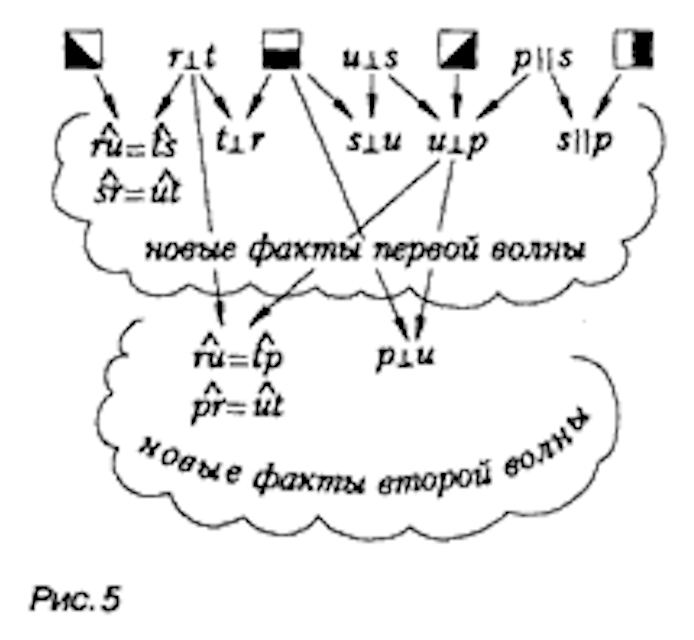
\includegraphics[scale=0.205]{images/IMG_20221205_213857_118.jpg}


\end{minipage}
\hspace{0.3cm}
\begin{minipage}{0.3\textwidth}

тех пор, пока не обнаружатся два противоречивых, взаимоисключающим факта -
они и будут сигнализировать об ошибочности исходного предположения.
  В реальных решающих <<интеллектуальных>> системах используются <<гибридные>> алгоритмы, в которых логический вывод органично сочетается с анализом информационных связей.

\vspace{0.3cm}
\hline
\vspace{0.09cm}
\large{
<<Мне бы ваши проблемы! >>
}
\hline
\vspace{0.15cm}

\small
\hspace{0.1cm}  -скажет machina sapiens в будущем, а сейчас она лишь делает первые шаги,чтобы разобраться в наших сложных житейских проблемах.

\hspace{0.1cm}   Разработчики машинного интеллекта
заметили, что логические модели, используемые при решении математических задач, с успехом могут быть применены к 
описанию широкого класса отношений:
родства, служебной подчиненности (между людьми), пространственных, временных, причинно-следственных (между различными объектами и процессами физического мира). Предлагаем читателю самостоятельно осуществить логический вывод, анализируя условие следующей
задачи:

\hspace{0.1cm}  <<Кухарка в Герцогиню метнула: банку,
склянку, вилку, ложку и неочищенную
картошку. Вилку она метнула позже банки, но не позже склянки, ложку - раньше склянки, но не позже банки. Восстановите последовательность брошенных пред-
метов, если неочищенная картошка предшествовала ложке и была пущена вслед за вилкой>>.

\hspace{0.1cm} В расследовании вышеописанного кухонного инцидента весьма полезными оказываются правила:


X позже Y $\rightarrow$ Y раньше X, 


X предшествует Y $\rightarrow$ X раньше Y, 


X вслед Y $\rightarrow$ Y раньше X, 


X раньше Y, Y раньше Z $\rightarrow$ X раньше Z.

\vspace{0.1cm}
\hspace{0.1cm} Переменные X, Y, Z здесь обозначают
произвольные объекты, в том числе и те, которые Кухарка в состоянии метнуть в Герцогиню.


\hspace{0.1cm} Человек, если это не связано с его
научной деятельностью, редко пользуется строгой математической логикой. В его
лексиконе нередки оценки: <<может быть>>, <<скорее всего>>,<<кажется>>, <<примерно>> и прочие, а вывод часто основывается на правдоподобных рассуждениях. Вот как,
например, рассуждает бармен в расска-
занной С.В. Чесноковым истории <<Силлогизм бабушки>>:


\hspace{0.1cm} << - Вы не правы, - к удивлению друзей
вежливо, но твердо возразил бармен. -
Еще моя покойная бабушка, помню, лю-


\noindent\rule{2cm}{0.4pt}


\scriptsize
1 В книге Д.А. Поспелова <<Моделирование рассуждений>> М.: Радио и связь. 1989.
  

\end{minipage}


\vspace{1cm}
\begin{center}
Пример работы с формулами 
  \begin{displaymath}
    \cos (\alpha) = \frac {b}{c}

    x_{i} = \frac {\sum_{j=1}^N x^{j}_{i}}{\sum_{i=1}^n x^{j}_{i} \sum_{j=1}^N x^{j}_{i}}
  \end{displaymath}
\end{center}

\vspace{1cm}
\begin{center}
    https://kvant.ras.ru/1994/03/Machina_sapiens.htm
\end{center}